% gm-16-SphericalTrigonometry.tex

\documentclass[xcolor=dvipsnames]{beamer}

\usepackage{tikz}
\usepackage{cancel}
\renewcommand{\CancelColor}{\color{red}}
\usepackage{graphicx}
\usepackage{wrapfig}
\usepackage{colortbl}
\usepackage{color}
\usepackage{alltt}
\renewcommand*{\thefootnote}{\fnsymbol{footnote}}
\definecolor{myblue}{rgb}{0.8,0.85,1}

\mode<presentation>
{
  \usetheme{Warsaw}
  \setbeamercovered{transparent}
}
% \usecolortheme[named=OliveGreen]{structure}
\setbeamertemplate{navigation symbols}{} 
\setbeamertemplate{blocks}[rounded][shadow=true] 

% this is for overlaying math symbols, see https://tex.stackexchange.com/questions/12895/overlay-symbol-with-another
\def\qeq{\mathrel{%
    \mathchoice{\QEQ}{\QEQ}{\scriptsize\QEQ}{\tiny\QEQ}%
}}
\def\QEQ{{%
    \setbox0\hbox{$\longrightarrow$}%
    \rlap{\hbox to \wd0{\hss/\hss}}\box0
  }}

\newcounter{expls}
\setcounter{expls}{0}
\newcommand{\beispiel}[1]{\refstepcounter{expls}\textbf{Example \arabic{expls}: #1.}}

\newcounter{exercise}
\setcounter{exercise}{0}
\newcommand{\ubung}[0]{\refstepcounter{exercise}\textbf{Exercise \arabic{exercise}: }}

\newif\ifBCITCourse
\BCITCoursetrue
% \BCITCoursefalse
\newif\ifWhichCourse
\WhichCoursetrue
\WhichCoursefalse
\ifBCITCourse
\ifWhichCourse
\newcommand{\CourseName}{Technical Mathematics for Food Technology}
\newcommand{\CourseNumber}{MATH 1441}
\newcommand{\CourseInst}{BCIT}
\else
\newcommand{\CourseName}{Technical Mathematics for Geomatics}
\newcommand{\CourseNumber}{MATH 1511}
\newcommand{\CourseInst}{BCIT}
\fi
\else
\newcommand{\CourseName}{Philosophy and Literature}
\newcommand{\CourseNumber}{PHIL 375}
\newcommand{\CourseInst}{UBC}
\fi

\title{Spherical Trigonometry}
\subtitle{{\CourseNumber}, BCIT}

\author{\CourseName}

\date{November 29, 2017}

\begin{document}

\begin{frame}
  \titlepage
\end{frame}

\begin{frame}
  \frametitle{Captain America I}
  \begin{quote}
    Realizing that in our present national emergency trigonometry is
    used in practically every phase of our war effort, the objective
    of the authors in writing this book was to present a brief but
    mathematically accurate course in plane and spherical trigonometry
    with special emphasis on the computational or practical side of
    the subject. In those chapters dealing with computational
    trigonometry, thorough drill is first given through the use of
    many examples.
  \end{quote}
\end{frame}

\begin{frame}
  \frametitle{Captain America II}
  \begin{quote}
    This is followed at the end of each of these chapters by practical
    applications introduced as problems, along with the necessary
    explanations and definitions, to secure conciseness of
    presentation. The applications deal with surveying, gun fire,
    course and position of airplanes, and navigation. This arrangement
    of theory and application in the book has permitted a sharp
    presentation of the underlying ideas which is necessary for rapid
    mastery of the subject. (Clifford Bell and Tracy Thomas,
    \emph{Essentials of Plane and Spherical Trigonometry}, 1943, page
    iii)
  \end{quote}
\end{frame}

\begin{frame}
  \frametitle{Fundamentals of Spherical Trigonometry}
  Consider a spherical triangle.
  \begin{figure}[h]
    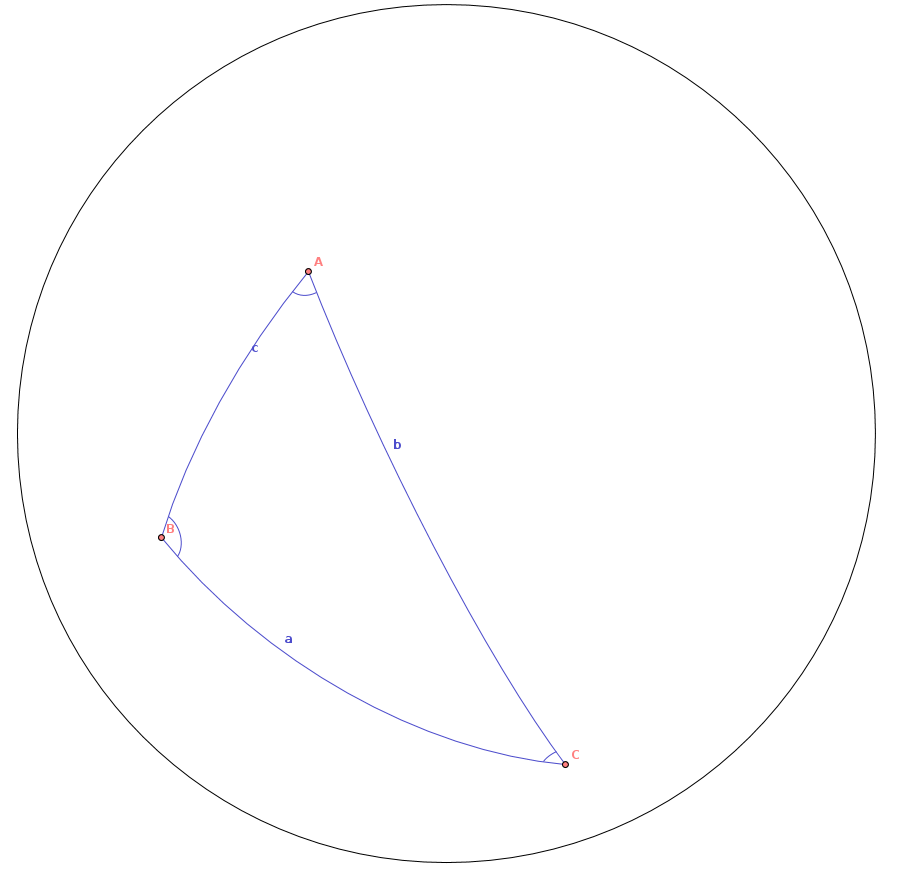
\includegraphics[scale=.25]{./SphericalTriangle.png}
  \end{figure}
\end{frame}

\begin{frame}
  \frametitle{Fundamentals of Spherical Trigonometry}
  Now notice that all sides of the spherical triangle correspond to
  angles at the centre of the sphere (in the diagram, the side $c$
  corresponds to the angle at $M$).
  \begin{figure}[h]
    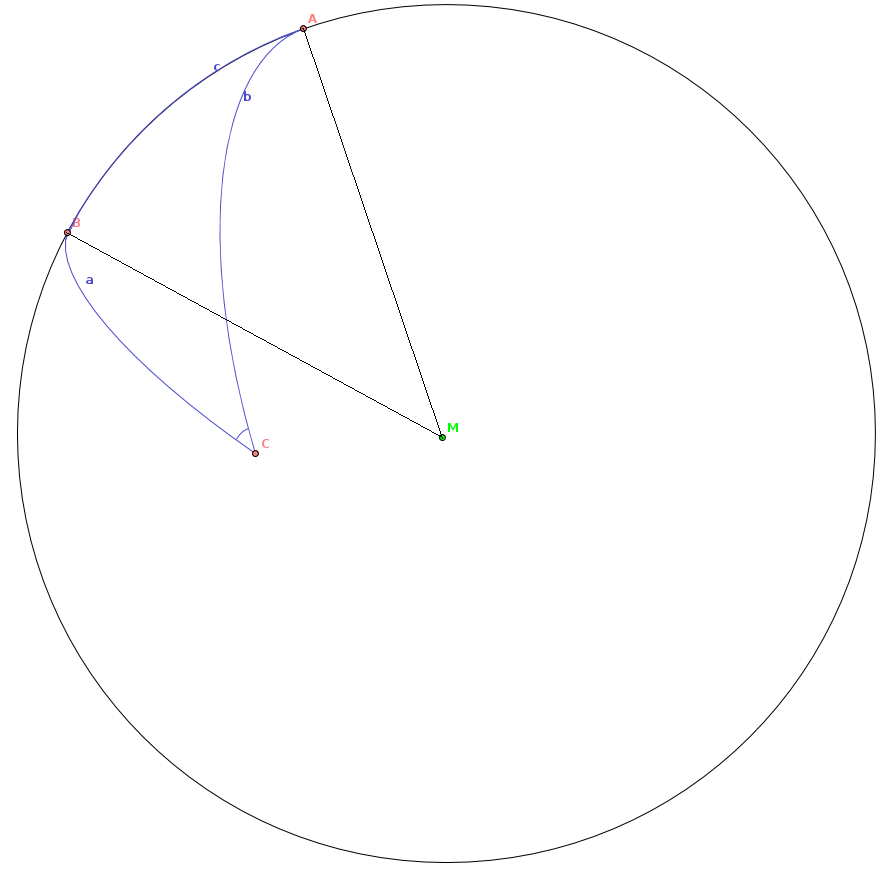
\includegraphics[scale=.2]{./sidesRangles.png}
  \end{figure}
\end{frame}

\begin{frame}
  \frametitle{Fundamentals of Spherical Trigonometry}
  In spherical trigonometry, sides are always given as angles. If you
  need to find the length, multiply by the radius. A side $\pi/4$
  ($45^{\circ}$) on the surface of the Earth, for example, has length
  \begin{equation}
    \label{eq:likashai}
    \frac{\pi}{4}\cdot{}6378.1km=5009.3km
  \end{equation}
  Three points on a sphere define eight different spherical triangles,
  depending on which way you loop around the sphere, the short way or
  the long way. We will always consider the triangle looping around
  the short way for all three sides. Therefore, all angles will be
  strictly between $0^{\circ}$ and $180^{\circ}$.
\end{frame}

\begin{frame}
  \frametitle{The Halifax Problem I}
This is a problem from Raymond Brink, \emph{Spherical Trigonometry},
1942, page 17.
\begin{quote}
  A ship leaves Halifax (position, $44.67^{\circ}N,63.58^{\circ}W$),
  starting due east [{\ldots}]. Find its
  position and direction after it has sailed 1000 nautical miles.
\end{quote}
\end{frame}

\begin{frame}
  \frametitle{The Halifax Problem II}
  \begin{figure}[h]
    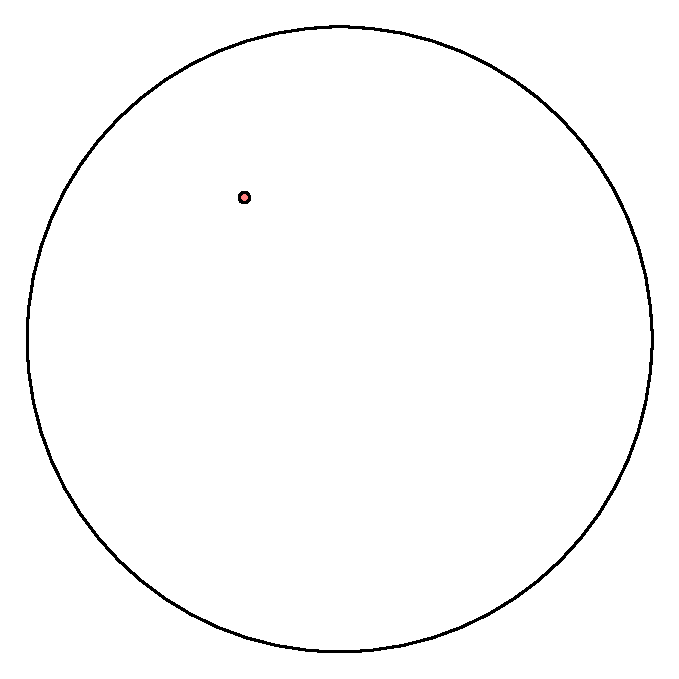
\includegraphics[scale=.7]{./bcita-01.eps}
  \end{figure}
\end{frame}

\begin{frame}
  \frametitle{The Halifax Problem III}
  \begin{figure}[h]
    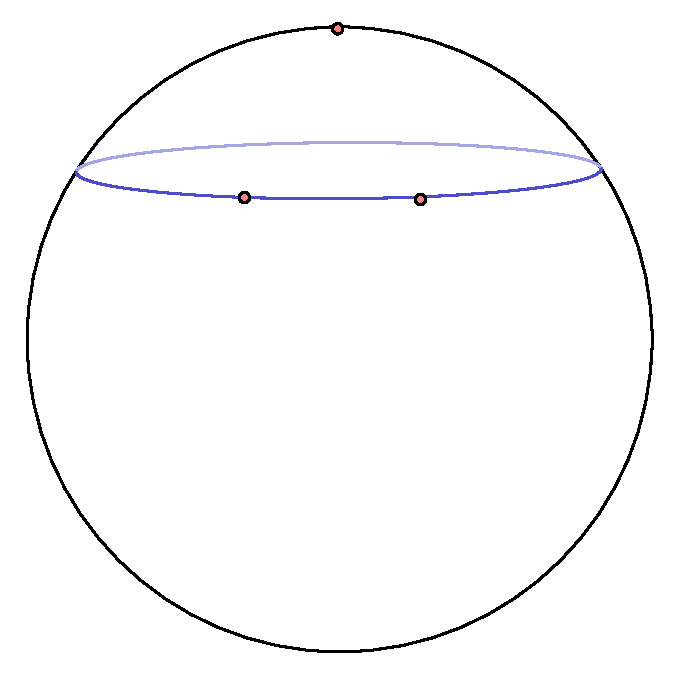
\includegraphics[scale=.7]{./bcita-02.eps}
  \end{figure}
\end{frame}

\begin{frame}
  \frametitle{The Halifax Problem IV}
  \begin{figure}[h]
    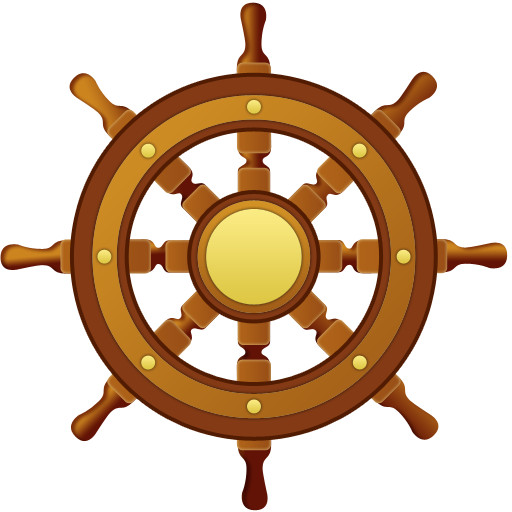
\includegraphics[scale=.4]{./wheel.jpg}
  \end{figure}
\end{frame}

\begin{frame}
  \frametitle{The Halifax Problem V}
  \begin{figure}[h]
    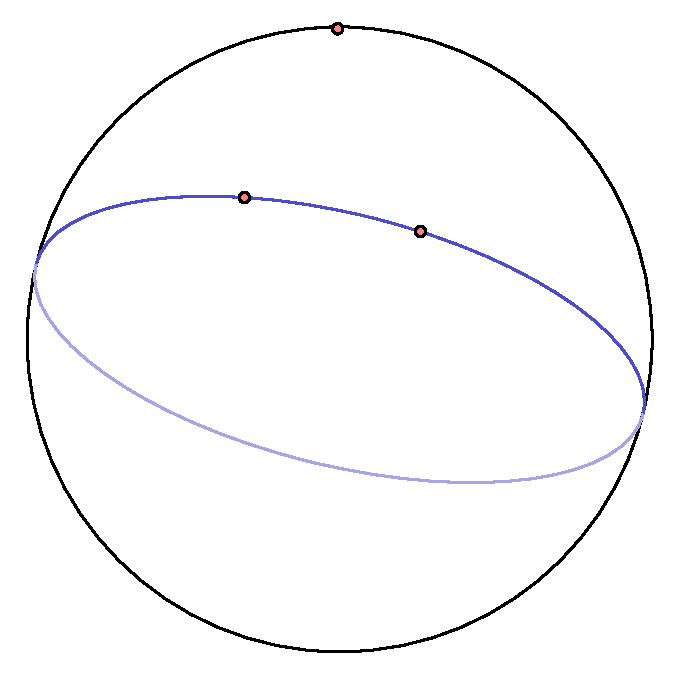
\includegraphics[scale=.7]{./bcita-03.eps}
  \end{figure}
\end{frame}

\begin{frame}
  \frametitle{The Halifax Problem IV}
This is a problem from Raymond Brink, \emph{Spherical Trigonometry},
1942, page 17.
\begin{quote}
  A ship leaves Halifax (position, $44.67^{\circ}N,63.58^{\circ}W$),
  starting due east \emph{and continuing on the great circle}. Find its
  position and direction after it has sailed 1000 nautical miles.
\end{quote}
\end{frame}

\begin{frame}
  \frametitle{Great Circles}
The intersection between a plane and a sphere is a circle. If the
centre of the sphere is an element of the plane, then the intersection
is a \alert{great circle}. A \alert{spherical angle} at point $P$ is
an arc length on a great circle for which $P$ is the pole.
\begin{block}{Triangle Sum}
  The sum of the angles of a spherical triangle is less than six right
  angles and greater than two right angles.
\end{block}
\end{frame}

\begin{frame}
  \frametitle{Napier's Pentagramma Mirificum}
\begin{figure} 
\centering 
\begin{minipage}{0.45\textwidth} 
\centering
    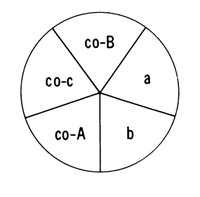
\includegraphics[scale=.8]{./nap1.png}
% \caption{first figure} 
\end{minipage}\hfill 
\begin{minipage}{0.45\textwidth} 
\centering 
    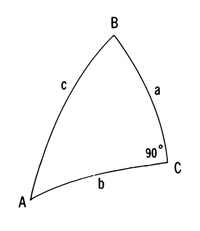
\includegraphics[scale=.8]{./nap2.png}
% \caption{second figure} 
\end{minipage} 
\end{figure} 
\end{frame}

\begin{frame}
  \frametitle{Napier's Rules}
  \begin{itemize}
  \item \emph{Rule I:} The sine of any circular part is equal to the
    product of the tangents of the two parts adjacent to it.
  \item \emph{Rule II:} The sine of any circular part is equal to the
    product of the cosines of the two parts opposite to it.
  \end{itemize}
\end{frame}

\begin{frame}
  \frametitle{The Right-Angled Euler Triangle I}
  \begin{figure}[h]
    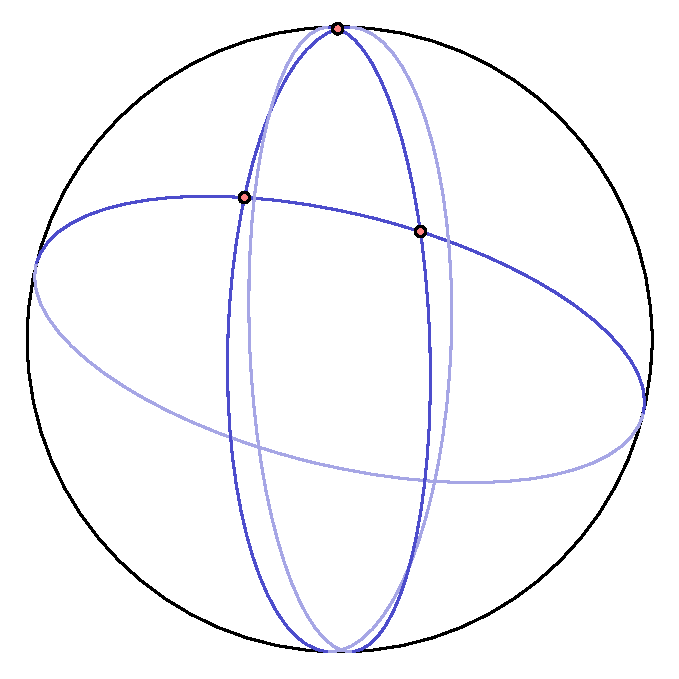
\includegraphics[scale=.7]{./bcita-04.eps}
  \end{figure}
\end{frame}

\begin{frame}
  \frametitle{The Right-Angled Euler Triangle II}
  \begin{figure}[h]
    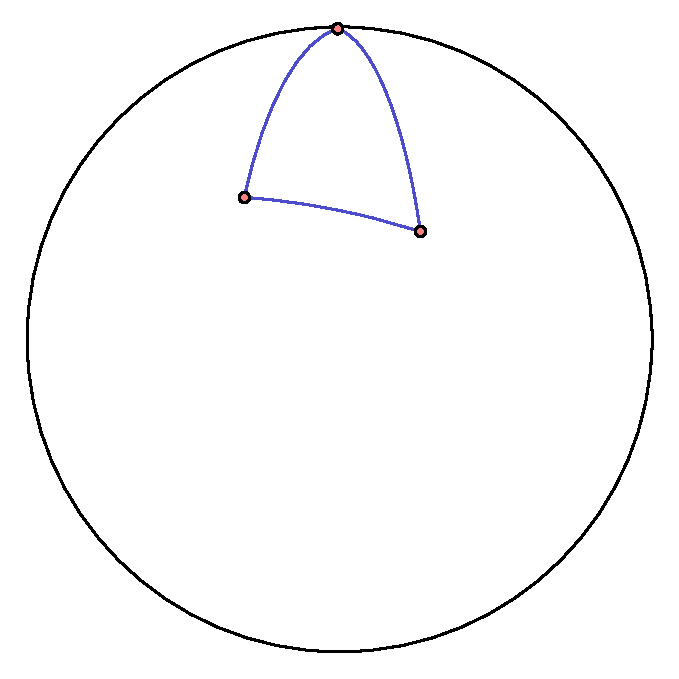
\includegraphics[scale=.7]{./bcita-05.eps}
  \end{figure}
\end{frame}

\begin{frame}
  \frametitle{Halifax Problem: Latitude}
Use the relevant three slices of the Pentagramma Mirificum for the
following formula:
\begin{equation}
  \label{eq:aeceiwae}
\cos{}c=\cos{}a\cdot\cos{}b  
\end{equation}
$a$ is 1000 nautical miles. One nautical mile is one minute of arc, or
$\frac{1}{60}^{\circ}$, on the Earth's surface. Therefore,
$a=16.667^{\circ}$ and $b=45.33^{\circ}$. Using the inverse function
of cosine on $\cos{}a\cdot\cos{}b$ and subtracting the result from
$90^{\circ}$, the result for the latitude of $E$ is $42.337^{\circ}N$.
\end{frame}

\begin{frame}
  \frametitle{Halifax Problem: Longitude}
Use the relevant three slices of the Pentagramma Mirificum for the
following formula:
\begin{equation}
  \label{eq:theeyoom}
\cos{}A=\cot{}c\cdot\tan{}b  
\end{equation}
Using the inverse function of cosine on $\cot{}c\cdot\tan{}b$ and
subtracting the result from $63.58^{\circ}$, the result for the
longitude of $E$ is $40.75^{\circ}W$.
\end{frame}

\begin{frame}
  \frametitle{Halifax Problem: Direction}
Use the relevant three slices of the Pentagramma Mirificum for the
following formula:
\begin{equation}
  \label{eq:cheichah}
\cos{}B=\cot{}c\cdot\tan{}a  
\end{equation}
Using the inverse function of cosine on $\cot{}c\cdot\tan{}a$, the
result for the direction at $E$ is $74.171^{\circ}$ east of south.
\end{frame}

\begin{frame}
  \frametitle{Exercises}
{\ubung} Remember this problem a while ago: 

\begin{block}{Windsor to Grenoble}
  Consider two towns, Windsor, Nova Scotia, at
  ($45^{\circ}N,65^{\circ}W$) and Grenoble, France at
  ($45^{\circ}N,5^{\circ}E$). If you follow a line of latitude, how
  far are the two towns apart?
\end{block}

We can now calculate the distance along the great circle.

\begin{figure}[h]
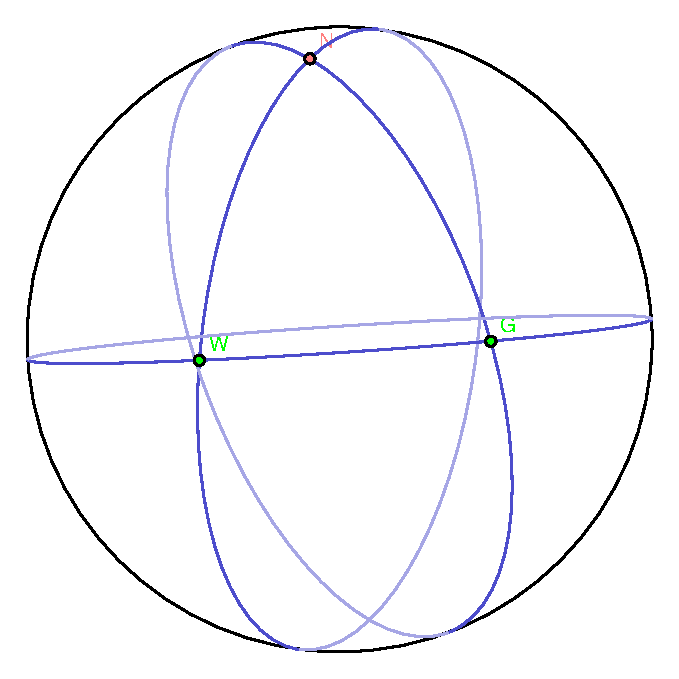
\includegraphics[scale=.3]{./WindsorGrenoble2.eps}
\end{figure}
\end{frame}

\begin{frame}
  \frametitle{Solution}
\begin{figure}[h]
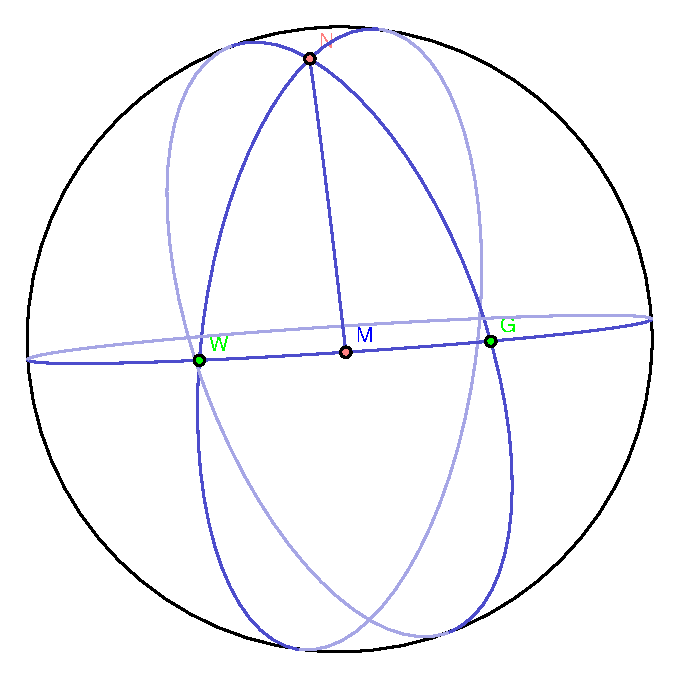
\includegraphics[scale=.55]{./WindsorGrenoble1.eps}
\end{figure}
\end{frame}

\begin{frame}
  \frametitle{Solution}
  $NWG$ is an isosceles triangle. Consequently, $NWM$ is a right
  triangle. Let $a=NM,b=MW,c=WN=45^{\circ}$. The angle $\angle{}WNM$
  is $35^{\circ}$. Napier's miraculous pentagram gives us
\begin{equation}
  \label{eq:yooceeva}
  \sin{}b=\sin{}35^{\circ}\cdot\sin{}45^{\circ}\mbox{ therefore }b=0.41761
\end{equation}
$b$ is in radians in equation (\ref{eq:yooceeva}). Multiply twice this
number by the radius of the Earth (6378.1km), and the correct solution
is approximately $5327.2$km, compared to approximately $5510.0$km
along the circle of latitude.

\bigskip

Note that the arcsine only gives us the
shorter of two solutions: we could also loop around the Pacific Ocean
instead of the Atlantic Ocean and get a much longer distance. The two
solutions add up to the circumference of the Earth.
\end{frame}

\begin{frame}
  \frametitle{Laws of Quadrants}
When you take the arcsine of a number on a calculator, the calculator
will always give you an angle less than $90^{\circ}$, for example the
arcsine of $\pi/4$ is $45^{\circ}$. However, the angle that you want
may be $135^{\circ}$, for $\sin{}135^{\circ}=\pi/4$ as well. The law
of quadrants helps you identify which angle (the acute or the obtuse)
you should accept as your solution.

\bigskip

Angles between $0^{\circ}$ and $90^{\circ}$ are considered to be in
the first quadrant. Angles between $90^{\circ}$ and $180^{\circ}$ are
considered to be in the second quadrant.
\end{frame}

\begin{frame}
  \frametitle{Law of Quadrants for Right Triangles}
For right spherical triangles,
  \begin{description}
  \item[LoQ I] An angle and its opposite side are in the same quadrant.
  \item[LoQ II] If any two of the three sides are in the same quadrant, the
    third side is in the first quadrant.
  \item[LoQ III] If any two sides are in different quadrants, the third side is
    in the second quadrant.
  \end{description}
\end{frame}

\begin{frame}
  \frametitle{Exercises}
% Clifford Bell, p136, ex. 1
{\ubung} One of the angles formed by the intersection of two great circles is
$37^{\circ}10'$. A point on one of the circles is $53^{\circ}27'$ from
the intersection point of the circles. Find the shortest distance from
this point to the other circle.
\begin{figure}[h]
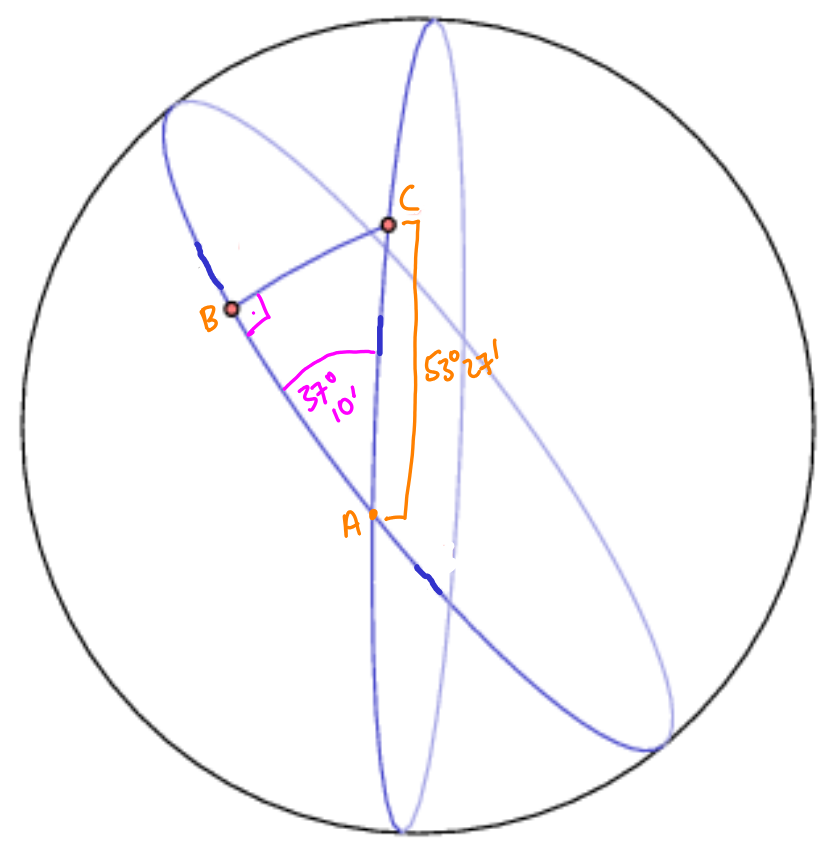
\includegraphics[scale=.3]{./cb.png}
\end{figure}
\end{frame}

\begin{frame}
  \frametitle{Exercises}
% Clifford Bell, p135
  {\ubung} Solve the isosceles triangle $ABC$, where $a=c=79^{\circ}17'$ and
  $A=C=59^{\circ}37'$.
\begin{figure}[h]
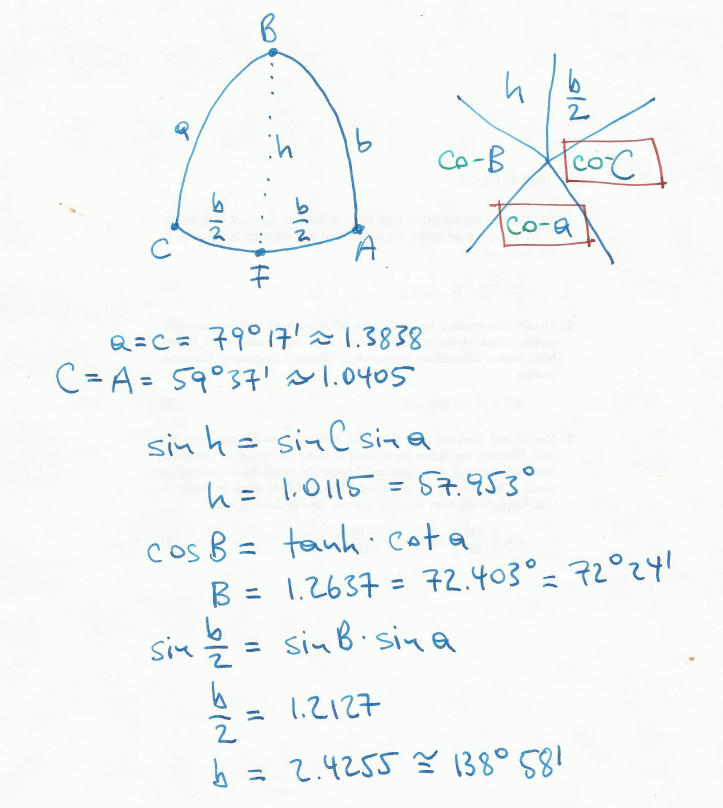
\includegraphics[scale=.25]{./gm-CliffordBell-p135-solution}
\end{figure}
\end{frame}

\begin{frame}
  \frametitle{Ambiguous Case}
  Consider the following problem.
  \begin{block}{Sailing from Lima}
    Your GPS is broken. You can only read your longitudes, but not
    your latitudes. You start from the Peruvian coast going west on a
    great circle at $77^{\circ}1'42''W$ and are now in the middle of
    the Pacific, having sailed 1750 nautical miles. Your longitude is
    $106^{\circ}44'27''W$. Where in Peru did you start (which town or
    city)?
  \end{block}
\end{frame}

\begin{frame}
  \frametitle{Ambiguous Case}
  \begin{figure}[h]
    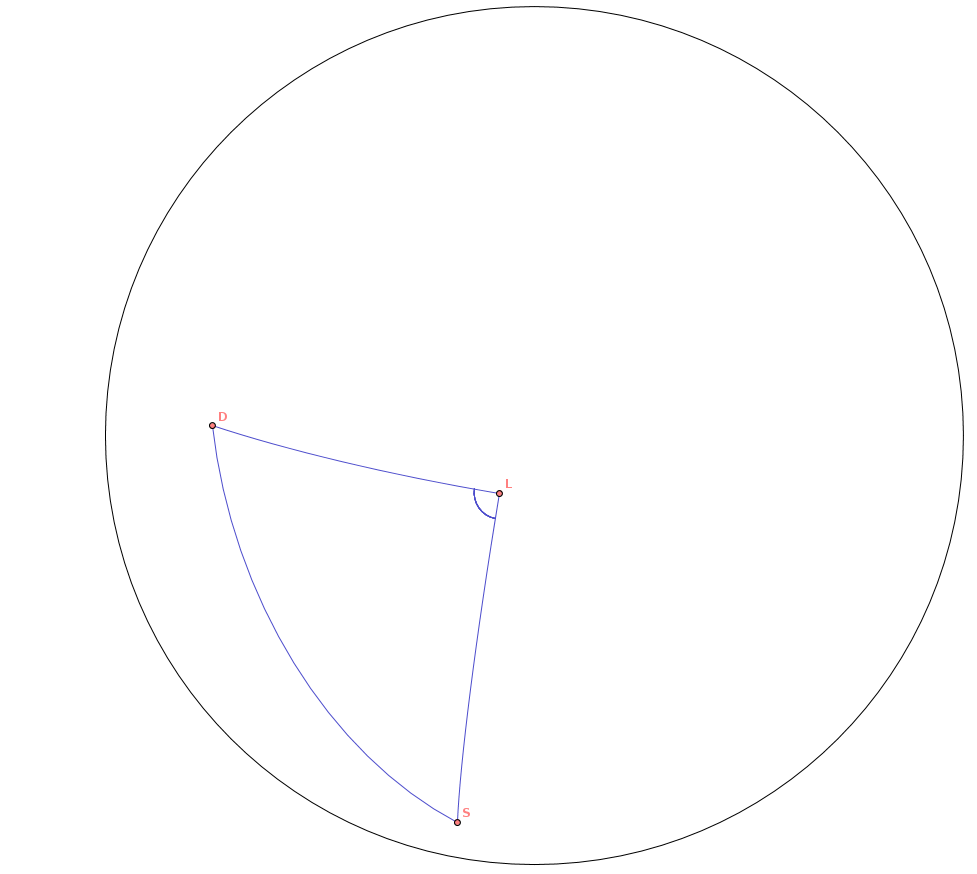
\includegraphics[scale=.25]{./rightamb.png}
  \end{figure}
\end{frame}

\begin{frame}
  \frametitle{Ambiguous Case}
  \begin{figure}[h]
    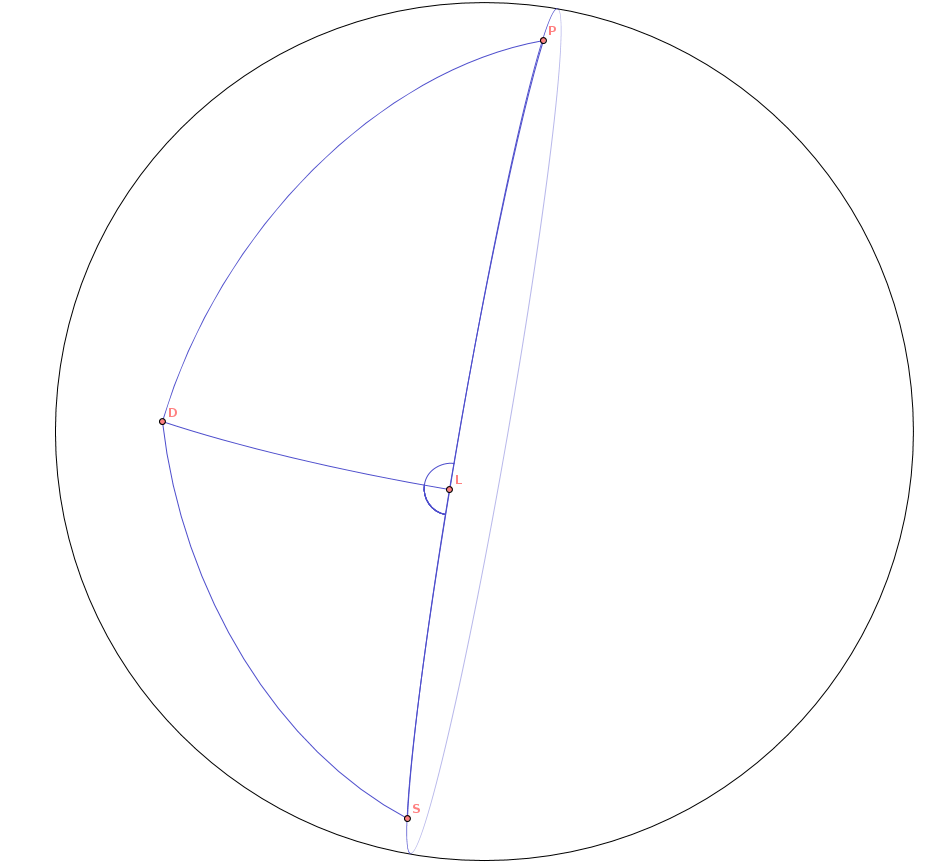
\includegraphics[scale=.25]{./rightamb1.png}
  \end{figure}
\end{frame}

\begin{frame}
  \frametitle{Ambiguous Case Answer}
Let the right angle be at $L$ and label it $C=90^{\circ}$. Label sides
$a,b,c$ and angles $A,B$ accordingly. We know $b=29.167^{\circ}$ and
$B=29.712^{\circ}$. The relevant law from Napier's miraculous
pentagram is
\begin{equation}
  \label{eq:saavooba}
  \sin{}a=\tan{}b\cdot\cot{}B
\end{equation}
It follows that $\sin{}a=0.97799$. There are two solutions for $a$.
\begin{equation}
  \label{eq:oongiemi}
  \begin{array}{rcl}
    a&=&77.957^{\circ} \\
    a&=&102.04^{\circ}
  \end{array}\notag
\end{equation}
In the context of the word problem, only the first solution makes
sense. The latitude of the origin is $12.043^{\circ}$, which on the
coast of Peru is the latitude for Lima.
\end{frame}

\begin{frame}
  \frametitle{Non-Right (Oblique) Spherical Triangles}
  Use the following three laws to solve non-right (oblique) spherical
  triangles.
  \begin{enumerate}
  \item Law of Sines
  \item Law of Cosines
  \item Napier's Analogies
  \end{enumerate}
\end{frame}

\begin{frame}
  \frametitle{Theorems of Spherical Trigonometry}
  The following theorems help to figure out which (if any) of the two
  arcsine solutions need to be rejected. I will call them oblique
  spherical triangle laws or OSTL in contrast to the Law of Quadrants
  for right spherical triangles. OSTL III is the law that does most of
  the heavy lifting.
  \begin{description}
  \item[OSTL I] The sum of the sides of a spherical triangle is less than
    $360^{\circ}$.
  \item[OSTL II] If two sides of a spherical triangle are equal, the angles
    opposite these sides are equal; and conversely.
  \item[OSTL III] If two sides of a spherical triangle are unequal, the angle
    opposite the greater side is the greater; and conversely.
  \end{description}
\end{frame}

\begin{frame}
  \frametitle{Polar Triangles}
  The three sides $a,b,c$ of a spherical triangle $D$ are arcs on a
  great circle. These three great circles have two poles each. Now
  choose three poles (one for each side) which determine a triangle
  such that all interior angles are strictly between $0^{\circ}$ and
  $180^{\circ}$. This new triangle $D'$ with sides $a',b',c'$ is
  called the \alert{polar triangle} of $D$. The polar triangle of $D'$
  is $D$ (in other words, $D''=D$). If $A,B,C$ are the angles of $D$
  and $A',B',C'$ are the angles of $D'$, then

  \bigskip

  \begin{tabular}{|rclcrcl|}\hline
    &&&\hspace{.5in}&&& \\
    $a+A'$&=&$180^{\circ}$&&$A+a'$&=&$180^{\circ}$ \\
    &&&\hspace{.5in}&&& \\
    $b+B'$&=&$180^{\circ}$&&$B+b'$&=&$180^{\circ}$ \\
    &&&\hspace{.5in}&&& \\
    $c+C'$&=&$180^{\circ}$&&$C+c'$&=&$180^{\circ}$ \\
    &&&\hspace{.5in}&&& \\ \hline
  \end{tabular}
\end{frame}

\begin{frame}
  \frametitle{Oblique Triangles Law of Cosines}
  Here is the cosine law for spherical triangles.
\begin{equation}
  \label{eq:epheepee}
  \cos{}a=\cos{}b\cos{}c+\sin{}b\sin{}c\cos{}A
\end{equation}
The corresponding cosine law for angles derived from the polar
triangle is
\begin{equation}
  \label{eq:dijeeghe}
  \cos{}A=-\cos{}B\cos{}C+\sin{}B\sin{}C\cos{}a
\end{equation}
\end{frame}

\begin{frame}
  \frametitle{Law of Cosines Example}
Calculate the distance along the great circle between Vancouver
($49^{\circ}15'$N, $123^{\circ}6'$W) and Palma de Mallorca
($39^{\circ}34'$N, $2^{\circ}39'$E).
\begin{figure}[h]
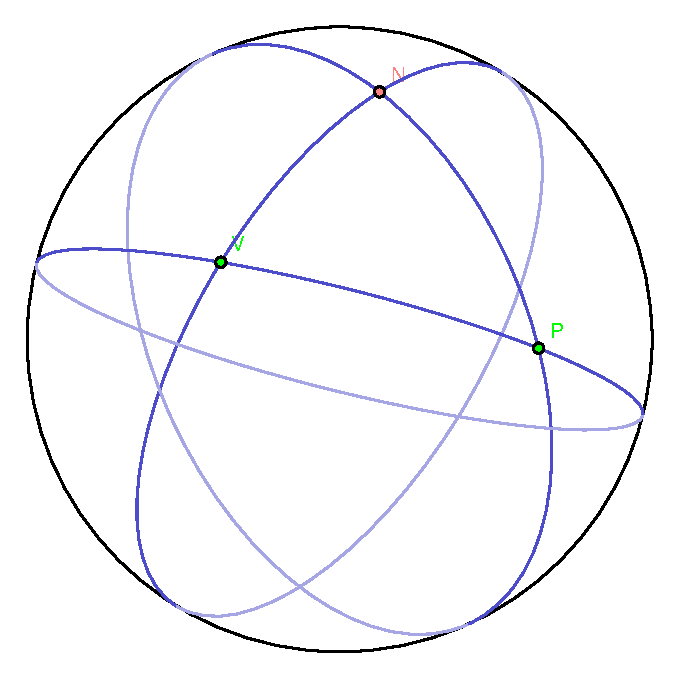
\includegraphics[scale=.4]{./VancouverPalma1.eps}
\end{figure}
\end{frame}

\begin{frame}
  \frametitle{Law of Cosines Example Solution}
\begin{figure}[h]
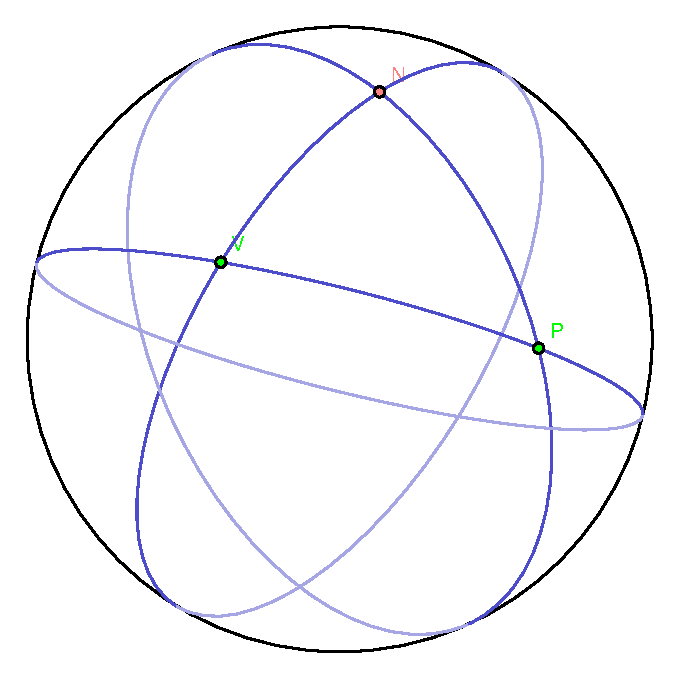
\includegraphics[scale=.4]{./VancouverPalma1.eps}
\end{figure}
Let $N$ be the angle $\angle{}VNP$. Let $a=VN,b=NP,c=VP$. According to
the law of cosines,
\begin{equation}
  \label{eq:aechiedu}
  \cos{}c=\cos{}a\cos{}b+\sin{}a\sin{}b{}cos{}N
\end{equation}
Consequently, $c=1.3811$ in radians, which translates to $8808.8$km.
\end{frame}

\begin{frame}
  \frametitle{Oblique Triangles Napier's Analogies}
Here are Napier's Analogies for oblique triangles. There is nothing
special about the labels $a,b,c$ and $A,B,C$. These analogies are true
for any permutation of $a,b,c$ and $A,B,C$, as long as it is
consistently applied. Note that $\sin\frac{1}{2}(a-b)$ means
$\sin[\frac{1}{2}(a-b)]$, not $\sin[\frac{1}{2}]\cdot{}(a-b)$.
\begin{equation}
  \label{eq:uteseivu}
  \begin{array}{l}
    \frac{\tan\frac{c}{2}}{\tan\left(\frac{1}{2}(a-b)\right)}=\frac{\sin\frac{1}{2}(A+B)}{\sin\frac{1}{2}(A-B)} \\
    \frac{\tan\frac{c}{2}}{\tan\left(\frac{1}{2}(a+b)\right)}=\frac{\cos\frac{1}{2}(A+B)}{\cos\frac{1}{2}(A-B)}
  \end{array}
\end{equation}
Napier's Analogies are helpful in roughly the same way the angle-sum
formula $\alpha+\beta+\gamma=180^{\circ}$ is helpful in plane
trigonometry.
\end{frame}

\begin{frame}
  \frametitle{Oblique Triangles Law of Sines}
  Here is the sine law for spherical triangles.
\begin{equation}
  \label{eq:aebaeyun}
  \frac{\sin{}a}{\sin{}A}=\frac{\sin{}b}{\sin{}B}=\frac{\sin{}c}{\sin{}C}
\end{equation}
The sine law usually gives you two solutions. Use OSTL III or the
cosine law to reject one of the two solutions.
\end{frame}

\begin{frame}
  \frametitle{ABC and Non-ABC}
  There are two types of oblique triangles.
  \begin{description}
  \item[ABC Type] If the knowns are ``ABC'', ``ABc'', ``AbC'', ``abC'', etc.,
    then the triangle is of the ABC type. Use the law of cosines first
    and then either the law of sines or Napier's Analogies.
  \item[Non-ABC Type] If the knowns are ``Aac'',``ABb'',``aCc'', etc., the
    triangle is of the non-ABC type. Use the law of sines first and
    then Napier's analogies (in plane trigonometry, you would use the
    law of sines and then the angle-sum formula).
  \end{description}
\end{frame}

% \begin{frame}
%   \frametitle{Things to Remember}
%   \begin{itemize}
%   \item In all the oblique triangle formulas (law of cosines, law of
%     sines, Napier's Analogies), the labels ``a'', ``b'', and ``c'' are
%     arbitrary, so they are also interchangable. You must apply these
%     changes consistently within the formula.
%   \item Using the law of cosines, law of sines, and Napier's Analogies
%     can saddle you with an incorrect solution. Always run all the sine
%     laws and all the cosine laws to check your solution.
%   \end{itemize}
% \end{frame}

\begin{frame}
  \frametitle{Spherical Trigonometry Decision Tree}
    \begin{figure}[h]
    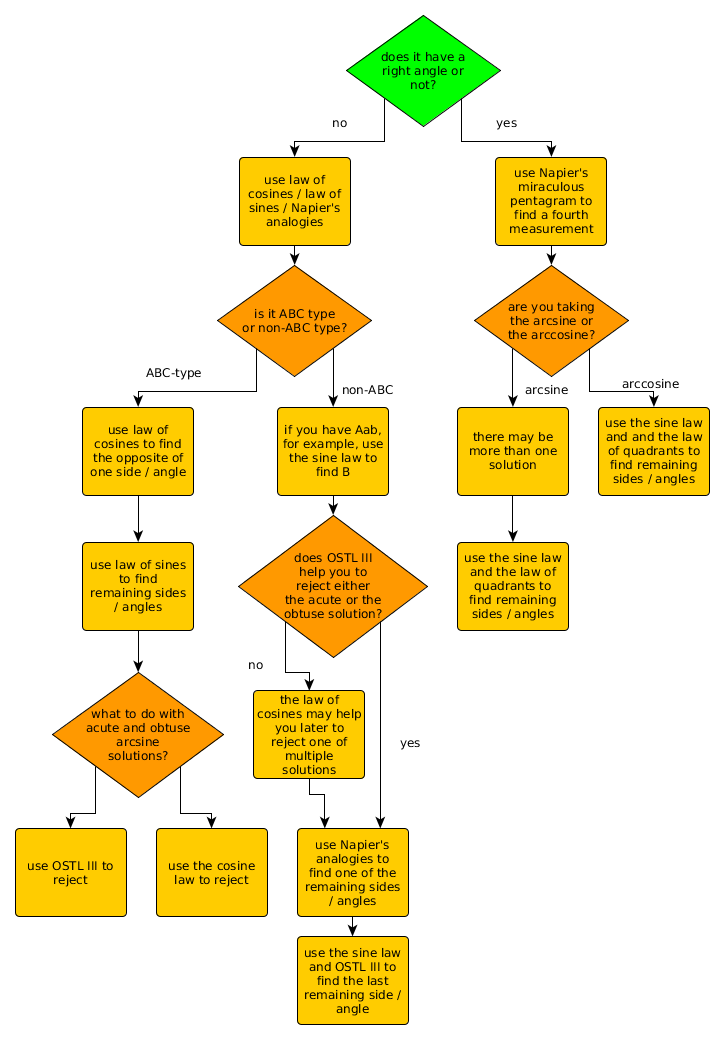
\includegraphics[scale=.25]{./sphericalTrig.png}
  \end{figure}
\end{frame}

% most of these exercises are from Welchons Krickenberger
\begin{frame}
  \frametitle{Exercises}
  {\ubung} Solve the following right spherical triangles:
  \begin{equation}
    \label{eq:dasohkoi}
    A=29^{\circ}11'\hspace{.5in}a=23^{\circ}56'     
  \end{equation}
  \begin{equation}
    \label{eq:eegaeboh}
    A=33^{\circ}20'\hspace{.5in}B=72^{\circ}40'     
  \end{equation}
  \begin{equation}
    \label{eq:enaigeos}
    a=126^{\circ}5'20''\hspace{.5in}A=105^{\circ}55'30''
  \end{equation}
\end{frame}

\begin{frame}
  \frametitle{Exercises}
  {\ubung} Solve the following right spherical triangles:
  \begin{equation}
    \label{eq:oosaelai}
    a=128^{\circ}12'10''\hspace{.5in}b=48^{\circ}56'20''
  \end{equation}
  \begin{equation}
    \label{eq:reethoht}
    A=79^{\circ}2'\hspace{.5in}a=72^{\circ}3'     
  \end{equation}
  \begin{equation}
    \label{eq:evieguso}
    a=75^{\circ}16'\hspace{.5in}b=130^{\circ}6'     
  \end{equation}
\end{frame}

\begin{frame}
  \frametitle{Exercises}
  {\ubung} Solve the following right spherical triangles:
  \begin{equation}
    \label{eq:aiwiphaj}
    B=84^{\circ}14'12''\hspace{.5in}b=78^{\circ}20'36'' 
  \end{equation}
  \begin{equation}
    \label{eq:ideichix}
    b=96^{\circ}20'45''\hspace{.5in}A=52^{\circ}8'30''
  \end{equation}
  \begin{equation}
    \label{eq:eeluyeeh}
    B=111^{\circ}42'\hspace{.5in}b=127^{\circ}35'     
  \end{equation}
\end{frame}

  % \begin{equation}
  %   \label{eq:ideichix}
  %   a=133^{\circ}21'\hspace{.5in}A=119^{\circ}28'     
  % \end{equation}

\begin{frame}
  \frametitle{Exercises}
  {\ubung} Solve the following isosceles spherical triangles:
  \begin{equation}
    \label{eq:aiyaawoo}
    A=B=80^{\circ}\hspace{.5in}C=110^{\circ}
  \end{equation}
  \begin{equation}
    \label{eq:cahghied}
    a=b=83^{\circ}12'50''\hspace{.5in}c=42^{\circ}24'10''
  \end{equation}
  \begin{equation}
    \label{eq:thaifahb}
    B=C=56^{\circ}56'\hspace{.5in}b=82^{\circ}12'
  \end{equation}
\end{frame}

\begin{frame}
  \frametitle{Exercises}
  {\ubung} Solve the following spherical triangles:
  \begin{equation}
    \label{eq:giezeoli}
    a=122^{\circ}18'\hspace{.5in}b=88^{\circ}21'\hspace{.5in}C=100^{\circ}16'    
  \end{equation}
  \begin{equation}
    \label{eq:vaibootu}
    a=44^{\circ}10'\hspace{.5in}b=18^{\circ}20'\hspace{.5in}A=64^{\circ}30'
  \end{equation}
  \begin{equation}
    \label{eq:ohjeegho}
    A=127^{\circ}20'\hspace{.5in}B=105^{\circ}40'\hspace{.5in}c=124^{\circ}30'
  \end{equation}
\end{frame}

\begin{frame}
  \frametitle{Exercises}
  {\ubung} Solve the following spherical triangles:
  \begin{equation}
    \label{eq:ciigahze}
    a=30^{\circ}40'\hspace{.5in}b=32^{\circ}30'\hspace{.5in}A=88^{\circ}2'
  \end{equation}
  \begin{equation}
    \label{eq:oozuufee}
    b=80^{\circ}5'\hspace{.5in}c=82^{\circ}55'\hspace{.5in}B=85^{\circ}12'
  \end{equation}
  \begin{equation}
    \label{eq:diepiemi}
    a=54^{\circ}20'\hspace{.5in}b=96^{\circ}40'\hspace{.5in}c=122^{\circ}18'
  \end{equation}
\end{frame}

\begin{frame}
  \frametitle{Exercises}
  {\ubung} Solve the following spherical triangles:
  \begin{equation}
    \label{eq:iexeenga}
    A=98^{\circ}16'\hspace{.5in}B=82^{\circ}24'\hspace{.5in}C=38^{\circ}48'    
  \end{equation}
  \begin{equation}
    \label{eq:oosheige}
    a=148^{\circ}12'\hspace{.5in}c=140^{\circ}33'\hspace{.5in}A=152^{\circ}45'
  \end{equation}
  \begin{equation}
    \label{eq:lahbeiro}
    a=96^{\circ}54'\hspace{.5in}B=82^{\circ}6'\hspace{.5in}c=104^{\circ}36'
  \end{equation}
\end{frame}

\begin{frame}
  \frametitle{Exercises}
  {\ubung} Find the length of the great-circle track from the Brooklyn
  Navy Yard ($40^{\circ}42'N,73^{\circ}59'W$) to the point where the
  prime meridian (the longitudinal circle that goes through Greenwich
  near London) crosses the equator.
\end{frame}

\begin{frame}
  \frametitle{Exercises}
  {\ubung} Find the length and the initial bearing of the great-circle
  track from Pearl Harbor ($21^{\circ}27'N, 157^{\circ}57'W$) to San
  Francisco ($37^{\circ}32'N,122^{\circ}13'W$).
\end{frame}

\begin{frame}
  \frametitle{Exercises}
  {\ubung} A ship sails from Boston ($42^{\circ}20'N, 70^{\circ}53'W$)
  to Lisbon ($38^{\circ}40'N,9^{\circ}18'W$). Find the distance of the
  great-circle track. Also find the bearing of the track when leaving
  Boston and when approaching Lisbon.
\end{frame}

\begin{frame}
  \frametitle{Exercises}
  {\ubung} Find the length of the shortest air route between Cape Town
  ($33^{\circ}56'S,18^{\circ}28'E$) and Dakar
  ($14^{\circ}40'N,17^{\circ}25'W$). What is the bearing of this
  track as the plane leaves Cape Town?
\end{frame}

\begin{frame}
  \frametitle{Exercises}
  {\ubung} Find the shortest distance between Greenwich ($51^{\circ}29'N$)
  and New York City ($40^{\circ}46'N,73^{\circ}51'W$). Also find the initial
  direction of the track.
\end{frame}

\begin{frame}
  \frametitle{Exercises}
  {\ubung} An airplane flies the great-circle track from Tokyo
  ($35^{\circ}39'N,139^{\circ}45'E$) to Wellington
  ($41^{\circ}17'S,174^{\circ}47'E$).
  \begin{enumerate}
  \item Find the length and initial direction of the great-circle
    track. 
  \item How far from Tokyo does the plane cross the equator and what 
is the longitude at the point of crossing? 
\item What is the bearing of the great-circle track as the plane
  crosses the equator?
  \end{enumerate}
\end{frame}

\begin{frame}
  \frametitle{Exercises}
  {\ubung} A plane leaves Chicago ($41^{\circ}50'N, 87^{\circ}36'W$)
  on a great-circle track with an initial bearing of $63^{\circ}30'$
  (counter-clockwise from east). What is the latitude and longitude of
  the plane after traveling 1000 nautical miles?
\end{frame}

\begin{frame}
  \frametitle{Exercises}
  {\ubung} If you were to make a nonstop flight from the city of
  Dayton, Ohio ($39^{\circ}46'N,84^{\circ}12'W$) to Tokyo
  ($35^{\circ}39'N,139^{\circ}45'E$) by the shortest route, in which
  direction would you start your flight?
\end{frame}

\begin{frame}
  \frametitle{Exercises}
  {\ubung} A plane leaves Los Angeles
  ($34^{\circ}3'N,118^{\circ}14'W$) on a great-circle track with an
  initial bearing of $65^{\circ}$. Find the latitude and longitude of
  the plane when it has flown 1000 nautical miles.
\end{frame}

\begin{frame}
  \frametitle{Exercises}

  {\ubung} What is the shortest distance from Moscow
  ($55^{\circ}43'N,37^{\circ}34'E$) to London ($51^{\circ}31'N,0^{\circ}6'W$)?
  Find the initial bearing of the track.
\end{frame}

% There are more exercises in gm-final-exam-mock.pdf from 2016

\begin{frame}
  \frametitle{End of Lesson}
Next Lesson: No Such Thing. Enjoy Your Holidays.
\end{frame}

\end{document}

% Find the shortest distance from Chicago (410 50' N, 8T 35' W) to Paris 
% (480 50' N, 20 20' E). 

% Find the shortest distance from New York (400 46' N, 730 51' W) 
% to Moscow (550 43' N, 380 34' E). 

% Find the distance and initial bearing of the shortest route from Rio 
% de Janeiro (220 54' S, 430 10' W) to Sydney (320 52' S, 1510 12' E). 


